
% View http://web.mit.edu/6.976/www/handout/valiant2.pdf

\section{Matrix algorithms}

While considering matrix algorithms, it is worth to consider the way the elements are laid out in memory. Sparse matrices are designed such that only non-zero entries are stored  as a triple of value and row, column. For a dense matrices, we usually distinguish the three following layouts:
\begin{itemize}
    \item Column major layout: The records are ordered by column first, and by row index within a column.
    \item Row major layout: The records are order row-wise first, and column-wise within a row.
    \item Recursive layout or zig-zag: Such layouts are often helpful to construct efficient cache-oblivious algorithm. Many applications involve (recursive) space filling curves to define the ordering of records.
\end{itemize}

\subsection{Matrix compaction and transposition}

The problem consists to transpose a matrix A of total size $N_{x} \times N_{y} = N$, composed as $P$ rows $A_{i}$ divided in $d$ sub-arrays, such that it procudes a new matrix $A^{'}$,
with $d$ rows and $P$ subdivisions. The segmentation is given through a matrix $M$ whose dimensions are 
$P \times d$ where $M[i, j]$ gives the size of the subarray.

A. Aggarwal and J. S. Vitter point out that transposition is a special case of permutation. Indeed, one can imagine that the matrix is broken down into several subgroups that will be used to create the final result. And then, it is necessary to merge the results through a fusion procedure, with the intuition that the same subgroups remain together. Hence a natural bound, for dense matrix, of $\Omega(\frac{N}{PB} \log_{d} \text{min}(B, N_{x}, N_{y}, \frac{N}{B}))$ with $d = \text{max}(2, \text{min}(\frac{M}{B}, \frac{N}{PB}))$~\cite{greiner2012sparse}. Cantazaro et al. propose another solution to this problem which has the advantage to be bank-conflict free~\cite{catanzaro2014decomposition}.

\begin{figure}[!htb]
    \centering
    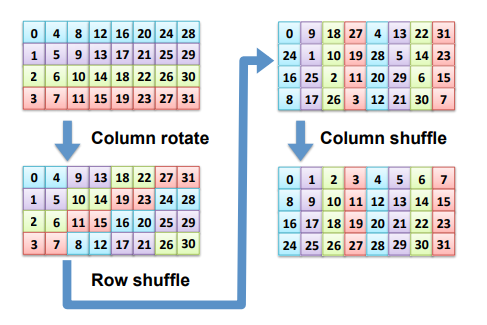
\includegraphics[width=0.8\linewidth]{Chapters/GPU/Algorithms/Transposition.png} 
    \caption{Catanzaro transposition - image extracted from Catanzaro et al.~\cite{nobile2014cutauleaping}, doi:10.1145/2692916.2555253}
\end{figure}

\subsection{Matrix-vector multiplication}

Performing a \textit{Sparse matrix-vector multiplication} can be bound in $\Omega(\frac{wH}{PB})$ with $H$ the number of non-empty entries and $w$ the number of vectors to multiply. And computing the bilinear form adds a factor of $O(\log ~ \text{min}(\frac{\sqrt{N}}{B}, \frac{P}{w}))$ since we can compute the partial scalar product when we are writing the resulting vector of the matrix multiplication and then gather the result~\cite{greiner2012sparse}. This extends the work of Bendal et al.~\cite{bender2010optimal} to parallel machines. Those sparse notions have a lot of application since they can have deep connection with graph problems~\cite{yang2015fast}.

\subsection{Matrix multiplication}

If we apply the standard matrix multiplication algorithm for two dense matrices, with the first matrix in row-major order and the second in column-major, for each element, we would have to do two scans, which would end up in $O(\frac{N^{3}}{PB})$ which is not optimal. Indeed, it is feasible to achieve $\Theta(\frac{N^{3}}{BP\sqrt{M}})$~\cite{ballard2012graph} for the classical algorithm, this coincides with one of the first result achieved by Hong and Kung. One should remark that multiple rows and columns are read several times, leading to inefficiency. The solution consists to store the elements of the matrices recursively, each time subdividing the 4 corners one after the other with a layout like $\text{layout}(Z) = \text{layout}(Z_{11})\text{layout}(Z_{12}) ... \text{layout}(Z_{22})$.

The complexity can be described by this system:
$$
\left\{
    \begin{array}{ll}
        MT(N) = 8MT(\frac{N}{2}) + O(\frac{N^{2}}{B}) \\
        MT(\sqrt{\frac{M}{3}}) = O(\frac{M}{B})
    \end{array}
\right.
$$

Indeed, each corner of the resulting matrix is obtained as the sum of the product of two sub-matrices, we have 4 corners with 2 products. The sums are independent of the recursion and cost $O(\frac{N^{2}}{B})$ since we scan along $X$ and $Y$. Finally, when the submatrices can be entirely contained in the cache\index{Cache}, and as they are stored continuously, the worst case is to go through all these blocks\index{Block}, $O(\frac{M}{B})$. Now, due to master theorem, we need to count the number of leaves, since the sum costs more than the recursion, there are thus $8^{\log N / \sqrt{M / 3}} = (N / \sqrt{M / 3})^{3}$ leaves. The total cost is finally:

$$ (\frac{N}{\sqrt{M / 3}})^{3} O(\frac{M}{B}) = \Theta(\frac{N^{3}}{M^{3/2}}) O(\frac{M}{B}) = \Theta(\frac{N^{3}}{B\sqrt{M}}) $$

%MT(N) = 8MT(N/2) + O(N^2 / B)
%Base case = MT(sqrt(M / 3)) => cost M/B
% There are 8^{log N / sqrt(M / 3)} leaves which is (N / sqrt(M / 3))
% Multilpy this by M / B
% https://youtu.be/CSqbjfCCLrU?t=1h16m53s


Sparse-dense matrix multiplication has a complexity dependent of the number of processors that we may offer, $\Omega(\frac{H\sqrt{N_{z}}}{PB\sqrt{M}})$ with $P \leq
HN_{z} / M^{\frac{3}{2}}$. Sparse-Sparse multiplication is still an open question, but we know that the complexity is bound by $\Omega(\frac{H_{1}H_{2}N}{PB} \log \frac{N}{\text{min}(H_{1}, H_{2}) B)})$ where $H_{1}$ (respectivelly $H_{2}$) is the average number of non-zero elements per column. Ballard et al.~\cite{ballard2011minimizing} regroup the results for the classical matrix decomposition (SVD, LU, ...).